\begin{figure}[H]
\centering
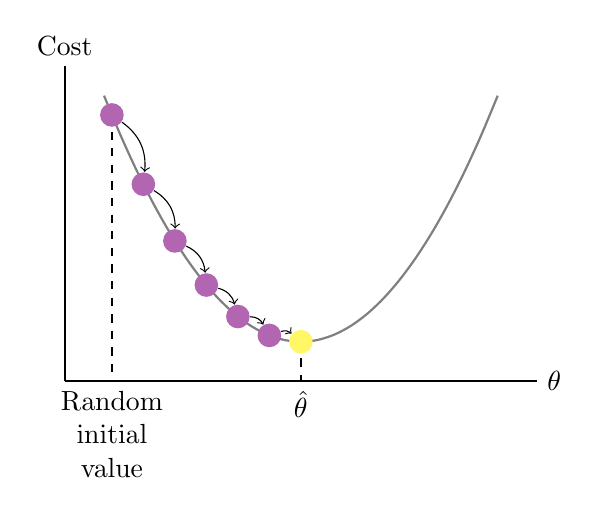
\begin{tikzpicture}[declare function={f(\x)=0.5*\x*\x-3*\x+5;}]
    \draw[thick](0,0)--(6,0) node[right]{$\theta$};
    \draw[thick,](0,0)--(0,4) node[above]{Cost};
    \draw[thick, dashed](0.6, {f(0.6)}) -- (0.6,0)
          node[below, text width=4em, align=center]{Random initial value};
    \draw[thick, dashed](3, {f(3)}) -- (3,0) node[below]{$\hat\theta$};
    \draw[domain=0.5:5.5, smooth, thick, gray] plot (\x, f(\x);
    \foreach \a [count=\c, remember=\c as \C] in {0.6, 1.0, ..., 2.6} {
      \node[circle, minimum size=3mm, inner sep=0pt, fill=violet!60] (\c) at (\a, {f(\a)}){};
      \ifnum\c>1
         \draw[->, bend left](\C) to (\c);
      \fi
    }
    \node[circle, minimum size=3mm, inner sep=0pt, fill=yellow!60] (Y) at (3, {f(3)}){}; 
    \draw[->, bend left](6) to (Y);
 \end{tikzpicture}
    \caption{Gradient descent method applied on a simple function.}
    \label{fig:grad-descent}
\end{figure}